\documentclass{beamer}

\usepackage[utf8]{inputenc}
\usepackage{graphicx}

\title{Recherche de chemin par dépôt de phéromones}
\author{Merwan Achibet}
\institute{Université du Havre}
\date{Jeudi 16 février 2012}

\usetheme{Warsaw}

\begin{document}

\maketitle

\section{Le modèle}

\begin{frame}

  \frametitle{Analogie avec le vivant}

  \begin{block}{}
    Les fourmis :
    \begin{itemize}
      \item{Fragiles, minuscules}
      \item{Une espèce pourtant très prospère}
    \end{itemize}
  \end{block}

  \vfill

  \begin{block}{Coopération $\rightarrow$ communication}
    Par des signaux chimiques, les phéromones
    \begin{itemize}
      \item{Piste vers une source de nourriture}
      \item{Délimitation d'un territoire}
      \item{Danger imminent}
      \item{Disposition à la reproduction}
    \end{itemize}
  \end{block}

\end{frame}

\begin{frame}

  \frametitle{Analogie avec le vivant}

  Les phéromones sont soumises à différents phénomènes naturels

  \begin{block}{L'évaporation}
    Elles sont éphémères et disparaissent progressivement
  \end{block}

  \begin{block}{La diffusion}
    Elles s'étalent dans l'espace
  \end{block}

  \begin{block}{Le renforcement}
    Leur puissance est renouvellée et augmentée par le passage d'autre
    individus.
  \end{block}

\end{frame}

\begin{frame}

  \frametitle{Qualités}

  \begin{itemize}
    \item[Diversité]{}
    \item[Distribution]{}
    \item[Décentralisation]{}
    \item[Dynamicité]{}
  \end{itemize}

\end{frame}

\begin{block}

  \frametitle{Dans le cadre militaire}

  \begin{itemize}
  \item{alentours de la fourmilière  $\rightarrow$ zone de conflit}
  \item{fourmis $\rightarrow$ drones aériens}
  \item{nourriture $\rightarrow$ bâtiments cibles}
  \item{dangers $\rightarrow$ bâtiments menaces}
  \end{itemize}

  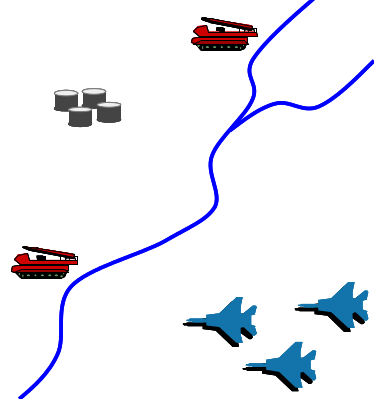
\includegraphics[width=3.5cm]{terrain_real.png}

\end{block}

\begin{block}

  \frametitle{Les phéromones}

  \begin{description}
  \item[GNest]{Mène à la base (le nid)}
  \item[GTarget]{Mène à une cible}
  \item[RTarget]{Libérée par les cibles, elle \textit{attire}}
  \item[RThreat]{Libérée par les menaces, elle \textit{repousse}}
  \end{description}

\end{block}

\begin{block}

  \frametitle{Guidage}

  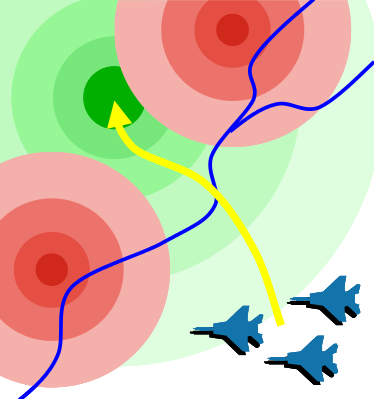
\includegraphics[width=3.5cm]{terrain_field.png}

  \begin{equation}
    g = \frac{ \theta \operatorname{RTarget} + \gamma \operatorname{GTarget} + \beta}{\alpha \operatorname{RThreat} + \delta \operatorname{Dist} + \beta}
  \end{equation}

\end{block}

\begin{block}

  \frametitle{Un nouveau type d'agent}

  \begin{block}{Les fantômes}
    \item{Courte durée de vie}
    \item{Haute vitesse}
  \end{block}

  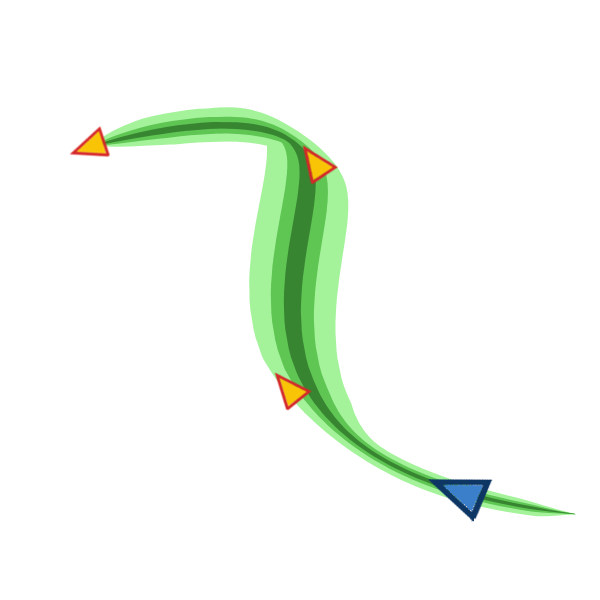
\includegraphics[width=3.5cm]{ghosts.png}

  Permet d'évaluer les chemins futurs

\end{block}

\section{L'implémentation}

\begin{block}

  \begin{block}
    \begin{itemize}
    \item{zones $\rightarrow$ patch}
    \item{agents $\rightarrow$ turtles}
    \end{itemize}
  \end{block}

  \begin{block}{La simulation}
    \begin{itemize}
    \item{Environnement aléatoirement généré}
    \item{Un unique drone}
    \item{objectif : atteindre une cible}
    \item{On ne se soucie pas du retour à la base}
    \end{itemize}
  \end{block}

\end{block}

\begin{block}

  IMAGES

\end{block}

\begin{block}

  \frametitle{Problème : un guidage trop simpliste}

  uphill

  La fonction d'évaluation de l'attractivité n'est pas utilisée

  $\rightarrow$ Nouvelle version

\end{block}

\begin{block}

  \frametitle{Fonctionnement}

  L'attractivité est mise à jour après chaque itération.

  \begin{enumerate}
  \item{Observer l'attractivité des huits zones voisines}
  \item{Tirage aléatoire sur une roue de la fortune biaisée}
  \item{Déplacement sur la case gagnante}
  \end{enumerate}

\end{block}

\begin{block}

  \frametitle{Influence des paramètres}

\end{block}

\begin{block}

  \frametitle{Influence des facteurs}

\end{block}

\end{document}
